\chapter{Des aimants d’Ising à la criticité liquide--gaz}

\lectureoverview{La transition liquide--gaz peut être abordée par une voie inattendue. Nous achevons d’abord le traitement en champ moyen de l’aimant d’Ising, repérons sa ligne de coexistence et son point critique, puis réinterprétons un spin orienté vers le haut comme un site occupé du réseau. Le gaz sur réseau qui en résulte présente une exclusion de cœur dur, une attraction à courte portée, un potentiel chimique contrôlé par le champ magnétique et exactement le même diagramme de phases. Le cours proprement dit s’achève sur le comportement critique et l’universalité. Une discussion distincte, après le cours, examine ensuite ce que les physiciens entendent par réglage fin, comment des effets de sélection peuvent intervenir dans une explication et pourquoi ce type de raisonnement n’est utile que s’il s’accompagne d’un mécanisme et de tests possibles.}

\section{Pourquoi l’étude de l’ébullition commence par un aimant}

L’ébullition de l’eau est le phénomène familier que nous voulons comprendre : un liquide devient un gaz et sa densité change brusquement. La démarche habituelle passe par l’équation de van der Waals. Ici, nous suivons une autre voie. Nous revenons à l’aimant d’Ising, achevons sa description en champ moyen, puis découvrons que le même modèle peut être interprété comme un fluide.

Il s’agit de bien plus qu’une analogie pittoresque. Une fois les variables correctement transposées, l’aimant d’Ising et le gaz sur réseau constituent le même système de mécanique statistique. L’aimantation devient la densité de particules, le champ magnétique extérieur devient un potentiel chimique, et la ligne de coexistence magnétique devient la ligne de coexistence liquide--gaz. Cette transposition explique pourquoi deux systèmes de matière apparemment différents peuvent présenter le même comportement critique.

En basse dimension, le champ moyen ne fournit pas de valeurs numériques exactes. En une dimension, il prédit même une transition que la solution exacte exclut. Son intérêt est ici structurel. En deux et trois dimensions, il révèle le bon paramètre d’ordre, les phases en compétition, l’extrémité critique et la manière dont un biais infinitésimal sélectionne une phase. En trois dimensions, où chaque site a six plus proches voisins, remplacer ces voisins par leur moyenne donne déjà une image qualitative utile.

\section{Le bilan énergétique du modèle d’Ising}

Plaçons un spin à deux états sur chaque site d’un réseau hypercubique,
\begin{equation}
\sigma_i=\pm1.
\end{equation}
Nous utilisons l’hamiltonien
\begin{equation}
\mathcal H
=-J\sum_{\langle ij\rangle}\sigma_i\sigma_j
+h\sum_i\sigma_i,
\qquad J>0.
\label{eq:ising-hamiltonian}
\end{equation}
La notation importe. La première somme porte sur les \emph{liaisons} entre plus proches voisins ; la seconde porte sur les \emph{sites}. Chaque liaison est comptée une fois, et non une fois depuis chacune de ses extrémités.

Pour une liaison,
\begin{equation}
E_{ij}=-J\sigma_i\sigma_j.
\end{equation}
Les spins parallèles ont une énergie \(-J\), tandis que les spins antiparallèles ont une énergie \(+J\). Une liaison rompue coûte donc
\begin{equation}
\Delta E_{\rm bond}=+J-(-J)=2J.
\label{eq:broken-bond}
\end{equation}
C’est la quantité \(2J\), et non l’une ou l’autre des énergies absolues de liaison, qui détermine les poids de Boltzmann relatifs. Nous pourrions ajouter une constante à chaque configuration sans modifier aucune probabilité.

\begin{classroomqa}
\audiencequestion{Pourquoi l’hamiltonien comporte-t-il deux sommes différentes ?}
\lecturerresponse{L’énergie d’échange concerne une paire de sites voisins ; elle est donc sommée sur les liaisons \(\langle ij\rangle\). Le champ agit indépendamment sur chaque spin ; il est donc sommé sur les sites \(i\). Confondre ces deux dénombrements introduit précisément les facteurs deux qui compteront en champ moyen. \lecturetimestamp{00:08:04--00:08:45}}
\end{classroomqa}

\begin{classroomqa}
\audiencequestion{Augmenter \(J\) rend-il simplement toutes les énergies plus négatives ?}
\lecturerresponse{Cela accroît l’écart entre les configurations alignées et désalignées. Le zéro de l’énergie est arbitraire ; l’énoncé physique est qu’une liaison rompue coûte \(2J\). Une valeur positive plus grande de \(J\) rend donc le désordre thermique moins favorable à température fixée. \lecturetimestamp{00:08:47--00:10:17}}
\end{classroomqa}

Sur un réseau hypercubique infini ou périodique en \(d\) dimensions, chaque site a \(2d\) voisins. Le dénombrement effectué à partir de chacun des \(N\) sites compte chaque liaison deux fois, d’où
\begin{equation}
N_{\rm links}=\frac{(2d)N}{2}=dN.
\label{eq:number-links}
\end{equation}
Une configuration alignée a donc une énergie d’échange égale à \(-JdN\). Les sites de bord modifient ce résultat par un terme de surface, négligeable devant \(N\) dans la limite thermodynamique. Les deux états complètement alignés sont dégénérés lorsque \(h=0\).

Le terme de champ fixe une convention de signe que nous conserverons de manière cohérente. Dans l’équation~\eqref{eq:ising-hamiltonian}, une valeur positive de \(h\) donne l’énergie de site la plus basse à \(\sigma=-1\). Ainsi, \(h>0\) favorise une aimantation négative, tandis que \(h<0\) favorise une aimantation positive. On peut inverser cette convention en écrivant \(-h\sum_i\sigma_i\) ; rien ne change physiquement, mais il faut alors inverser tous les signes qui suivent.

\begin{classroomqa}
\audiencequestion{Où intervient la température si l’hamiltonien ne contient que \(J\) et \(h\) ?}
\lecturerresponse{La température intervient par le facteur de Boltzmann \(e^{-\beta\mathcal H}\), avec \(\beta=1/T\) en unités \(k_{\rm B}=1\). Les grandeurs sans dimension sont donc \(\beta J\) et \(\beta h\). \lecturetimestamp{00:13:07--00:13:43}}
\end{classroomqa}

\section{Un spin dans le champ moyen de ses voisins}

Choisissons un spin loin du bord. Il a \(2d\) plus proches voisins. Le champ moyen remplace chaque voisin fluctuant par la même valeur moyenne
\begin{equation}
m=\expect{\sigma}.
\end{equation}
L’énergie d’échange faisant intervenir le spin choisi \(\sigma\) devient alors
\begin{equation}
-J\sigma\sum_{\text{\(2d\) neighbors}}\sigma_j
\;\longrightarrow\;-2dJm\,\sigma.
\end{equation}
En ajoutant le champ extérieur, on obtient l’énergie effective du spin unique
\begin{equation}
\mathcal H_{\rm mf}(\sigma)=(-2dJm+h)\sigma.
\label{eq:mean-field-one-spin}
\end{equation}
Le facteur \(2d\) est essentiel. Il est facile de l’omettre lorsqu’on écrit le schéma du spin central ; il a été rétabli explicitement pendant la dérivation au tableau.

\begin{figure}[ht]
\centering
\includegraphics[width=0.84\textwidth]{lecture_10_figure_02.png}
\caption{Un spin central entouré de ses voisins en champ moyen, avec l’énergie d’un spin et l’équation d’autocohérence en cours d’établissement.}
\lectureframe{00:17:57}
\end{figure}

La fonction de partition d’un spin est
\begin{align}
z_{\rm mf}
&=\sum_{\sigma=\pm1}
\exp\!\left[-\beta(-2dJm+h)\sigma\right] \\
&=2\cosh\!\left[\beta(2dJm-h)\right].
\end{align}
Son spin moyen vaut
\begin{align}
\expect{\sigma}
&=\frac{\sum_{\sigma=\pm1}\sigma
 e^{\beta(2dJm-h)\sigma}}
{\sum_{\sigma=\pm1}e^{\beta(2dJm-h)\sigma}} \\
&=\tanh\!\left[\beta(2dJm-h)\right].
\end{align}
Mais le spin choisi est censé être représentatif des voisins dont la moyenne a été notée \(m\). La condition d’autocohérence impose donc
\begin{equation}
\boxed{m=\tanh\!\left[\beta(2dJm-h)\right].}
\label{eq:mean-field-self-consistency}
\end{equation}
Cette unique équation non linéaire constitue la réduction en champ moyen du problème à plusieurs spins.

\begin{classroomqa}
\audiencequestion{Pourquoi la moyenne à gauche est-elle le même \(m\) que celui qui a été attribué à chaque voisin ?}
\lecturerresponse{Cette égalité est précisément l’approximation. Nous supposons un état homogène dans le volume, remplaçons l’environnement réel par sa moyenne, calculons le spin central dans cet environnement, puis exigeons que la moyenne calculée reproduise l’environnement supposé. Une solution est un état homogène autocohérent. \lecturetimestamp{00:16:28--00:18:00}}
\end{classroomqa}

Introduisons
\begin{equation}
y=2\beta dJm.
\label{eq:y-definition}
\end{equation}
Puisque \(\beta=1/T\),
\begin{equation}
m=\frac{yT}{2dJ},
\end{equation}
l’équation~\eqref{eq:mean-field-self-consistency} devient
\begin{equation}
\boxed{\frac{yT}{2dJ}=\tanh(y-\beta h).}
\label{eq:reduced-mean-field}
\end{equation}

\begin{figure}[ht]
\centering
\includegraphics[width=0.82\textwidth]{lecture_10_figure_03.png}
\caption{L’équation d’autocohérence réduite après introduction de \(y=2\beta dJm\), prête à être résolue graphiquement.}
\lectureframe{00:24:42}
\end{figure}

\begin{classroomqa}
\audiencequestion{Pourquoi le champ apparaît-il sous la forme \(y-\beta h\), et quel spin un champ positif favorise-t-il ?}
\lecturerresponse{Notre hamiltonien contient \(+h\sigma\). Son exposant de Boltzmann est donc \(\beta(2dJm-h)\sigma\), et la tangente hyperbolique comporte ainsi \(y-\beta h\). Une valeur positive de \(h\) favorise \(\sigma=-1\). Si l’on définissait plutôt l’hamiltonien avec \(-h\sigma\), chaque occurrence de \(h\) changerait de signe et le diagramme de phases serait réfléchi horizontalement. \lecturetimestamp{00:18:17--00:20:00}}
\end{classroomqa}

\section{Solutions graphiques et point de Curie}

Posons \(h=0\). Il faut trouver les intersections de
\begin{equation}
\frac{T}{2dJ}y
\qquad\text{and}\qquad
\tanh y.
\end{equation}
La première courbe est une droite passant par l’origine ; la seconde est une courbe impaire qui tend vers des valeurs limites. À haute température, la droite est pentue et l’unique intersection est \(y=0\), d’où \(m=0\). Lorsque la température baisse, la droite devient moins pentue. La température critique est atteinte lorsque la droite et la tangente hyperbolique sont tangentes à l’origine.

\begin{figure}[ht]
\centering
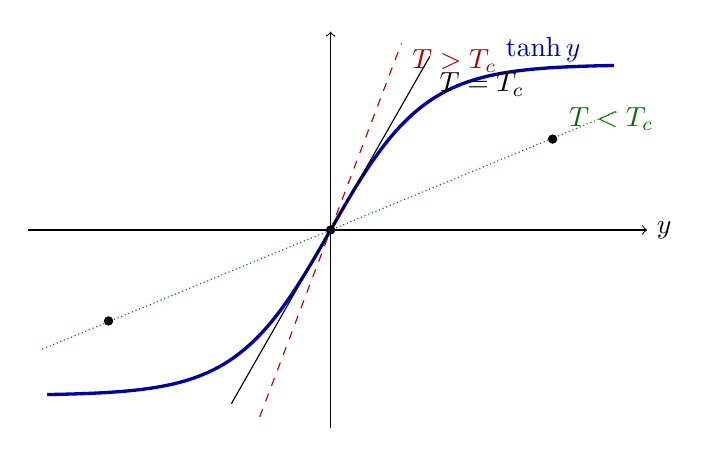
\begin{tikzpicture}[x=1.2cm,y=2.1cm]
\draw[->] (-3.2,0) -- (3.35,0) node[right] {$y$};
\draw[->] (0,-1.2) -- (0,1.2);
\draw[very thick,blue!65!black,domain=-3:3,samples=120]
  plot (\x,{tanh(\x)});
\node[blue!65!black,above] at (2.25,0.96) {$\tanh y$};
\draw[dashed,red!70!black] (-0.75,-1.13) -- (0.75,1.13);
\node[red!70!black,right] at (0.76,1.02) {$T>T_c$};
\draw[black] (-1.05,-1.05) -- (1.05,1.05);
\node[right] at (1.05,0.88) {$T=T_c$};
\draw[densely dotted,green!45!black] (-3.05,-0.72) -- (3.05,0.72);
\node[green!45!black,right] at (2.42,0.67) {$T<T_c$};
\fill (-2.35,-0.55) circle (1.7pt);
\fill (0,0) circle (1.7pt);
\fill (2.35,0.55) circle (1.7pt);
\end{tikzpicture}
\caption{L’équation de champ moyen à champ nul. En dessous de \(T_c\), les deux intersections non nulles représentent les phases aimantées stables ; la solution nulle reste présente algébriquement, mais elle est instable.}
\label{fig:mean-field-intersections}
\end{figure}

Comme
\begin{equation}
\left.\frac{d}{dy}\tanh y\right|_{y=0}=1,
\end{equation}
la condition de tangence est
\begin{equation}
\frac{T_c}{2dJ}=1.
\end{equation}
Le champ moyen prédit donc
\begin{equation}
\boxed{T_c^{\rm MF}=2dJ.}
\label{eq:sm10-mean-field-tc}
\end{equation}
En dessous de cette température, il existe deux solutions stables non nulles \(\pm m_0(T)\). La solution \(m=0\) satisfait toujours l’équation, mais elle n’est plus un équilibre stable. Le système choisit l’une des deux phases aimantées liées par symétrie.

\begin{classroomqa}
\audiencequestion{Est-ce la température de Curie ?}
\lecturerresponse{Oui. Pour un ferromagnétique, la température à laquelle l’aimantation spontanée disparaît est appelée conventionnellement température de Curie. Ici, \(2dJ\) en est la valeur en champ moyen, et non un résultat exact en basse dimension. \lecturetimestamp{00:28:19--00:28:57}}
\end{classroomqa}

Au voisinage de la transition, développons la tangente hyperbolique :
\begin{equation}
\tanh y=y-\frac{y^3}{3}+O(y^5).
\end{equation}
Pour \(h=0\), l’équation~\eqref{eq:reduced-mean-field} donne
\begin{equation}
\left(1-\frac{T}{T_c}\right)y-\frac{y^3}{3}+O(y^5)=0.
\end{equation}
Les branches non nulles se comportent donc comme
\begin{equation}
y^2\simeq3\left(1-\frac{T}{T_c}\right),
\qquad
m\propto(T_c-T)^{1/2}.
\label{eq:mf-beta-exponent}
\end{equation}
La racine carrée définit un exposant critique de champ moyen. Sa valeur précise ne sera pas conservée en basse dimension, mais le paramètre d’ordre s’annulera continûment à l’extrémité.

\section{Le plan température--champ et le choix des branches}

Le matériau fixe \(J\) ; l’expérimentateur peut faire varier \(T\) et \(h\). Il est donc naturel de tracer un diagramme de phases dans le plan \(T\)--\(h\). En dessous de \(T_c\), un champ arbitrairement faible sélectionne l’une des deux branches aimantées. Avec notre convention, \(h<0\) sélectionne \(m>0\), tandis que \(h>0\) sélectionne \(m<0\).

À température nulle, les spins sont complètement alignés, donc \(m=\pm1\). À haute température, la moyenne à champ nul vaut \(m=0\). Lorsqu’on s’approche du point critique le long de \(h=0\), la valeur absolue de \(m_0(T)\) décroît continûment jusqu’à zéro. Mais à \(T<T_c\) fixé, traverser \(h=0\) provoque le passage discontinu de \(+m_0(T)\) à \(-m_0(T)\).

\begin{figure}[ht]
\centering
\includegraphics[width=0.90\textwidth]{lecture_10_figure_06.png}
\caption{La ligne de coexistence dans le plan \(T\)--\(h\) et les branches d’aimantation à température fixée en dessous de \(T_c\).}
\lectureframe{00:39:30}
\end{figure}

\begin{figure}[ht]
\centering
\resizebox{\linewidth}{!}{%
\begin{tikzpicture}[x=1.25cm,y=1.15cm]
\begin{scope}
\draw[->] (-2.45,0) -- (2.55,0) node[right] {$h$};
\draw[->] (0,0) -- (0,3.7) node[above] {$T$};
\draw[very thick,red!70!black] (0,0) -- (0,2.35);
\fill[red!70!black] (0,2.35) circle (2.3pt);
\node[right] at (0.08,2.35) {$T_c$};
\node at (-1.25,1.05) {$m>0$};
\node at (1.25,1.05) {$m<0$};
\draw[->,rounded corners,blue!65!black] (-1.65,0.85) -- (-1.65,3.02)
 -- (1.65,3.02) -- (1.65,0.85);
\node[blue!65!black] at (0,3.35) {continuous path};
\end{scope}
\begin{scope}[xshift=7.0cm,yshift=1.55cm]
\draw[->] (-2.5,0) -- (2.5,0) node[right] {$h$};
\draw[->] (0,-1.35) -- (0,1.4) node[above] {$m$};
\draw[very thick,blue!65!black]
  (-2.2,1.05) .. controls (-0.75,1.03) and (-0.2,0.75) .. (-0.08,0.62);
\draw[very thick,blue!65!black]
  (0.08,-0.62) .. controls (0.2,-0.75) and (0.75,-1.03) .. (2.2,-1.05);
\draw[dashed] (0,0.62) -- (0,-0.62);
\fill (0,0.62) circle (1.8pt);
\fill (0,-0.62) circle (1.8pt);
\node at (0,-1.75) {\(T<T_c\)};
\end{scope}
\end{tikzpicture}
}
\caption{À \(T<T_c\) fixé, l’aimantation saute lorsqu’on traverse la ligne de coexistence. Dans le plan complet des deux paramètres, on peut au contraire relier continûment les deux phases en contournant le point critique.}
\label{fig:ising-phase-plane}
\end{figure}

\begin{classroomqa}
\audiencequestion{Que se passe-t-il si le champ est exactement nul en dessous de \(T_c\) ?}
\lecturerresponse{Le système idéal infini possède deux phases pures également favorables. Tout biais résiduel infinitésimal, toute condition aux limites ou toute fluctuation liée à la préparation en sélectionne une. La discontinuité thermodynamique s’exprime par les deux limites unilatérales \(m(T,0^-)=+m_0(T)\) et \(m(T,0^+)=-m_0(T)\), selon notre convention de signe. \lecturetimestamp{00:35:04--00:37:10}}
\end{classroomqa}

\begin{classroomqa}
\audiencequestion{Est-ce la même chose que l’hystérésis ?}
\lecturerresponse{L’hystérésis concerne la métastabilité et le retard dépendant de l’histoire avec lequel un système réel passe d’une branche à l’autre. Le phénomène est lié, mais nécessite une dynamique qui dépasse le diagramme de phases à l’équilibre ; nous ne l’étudierons pas ici. \lecturetimestamp{00:37:11--00:37:20}}
\end{classroomqa}

\begin{classroomqa}
\audiencequestion{Peut-on relier les phases positive et négative sans traverser de discontinuité ?}
\lecturerresponse{Oui. Élevons la température au-dessus de \(T_c\), changeons-y le signe du champ, puis abaissons de nouveau la température. Ce parcours contourne l’extrémité et l’aimantation varie continûment. Le saut est inévitable uniquement si l’on traverse \(h=0\) à \(T<T_c\) fixé. \lecturetimestamp{00:37:20--00:38:15}}
\end{classroomqa}

\begin{classroomqa}
\audiencequestion{L’aimantation tend-elle vers zéro chaque fois que \(h\) tend vers zéro ?}
\lecturerresponse{Pas à une température quelconque inférieure à \(T_c\). Les limites unilatérales y sont non nulles. L’aimantation spontanée ne tend vers zéro que lorsque la température critique elle-même est approchée. \lecturetimestamp{00:38:29--00:39:45}}
\end{classroomqa}

\section{Une enceinte perméable et le potentiel chimique}

Nous délaissons maintenant les aimants et reprenons notre étude avec des particules. Imaginons une région dont l’énergie potentielle est inférieure à celle de l’espace environnant. Les parois sont perméables : les particules peuvent entrer et sortir. Si l’énergie intérieure est inférieure de \(\mu\), l’occupation de l’enceinte reçoit un facteur de Boltzmann relatif \(e^{\beta\mu}\). Approfondir ou relever le puits modifie le nombre moyen de particules dans l’enceinte.

\begin{figure}[ht]
\centering
\includegraphics[width=0.84\textwidth]{lecture_10_figure_07.png}
\caption{Représentation d’une enceinte perméable par un puits de potentiel. La différence d’énergie entre l’intérieur et l’extérieur détermine la préférence des particules pour l’occupation de l’enceinte.}
\lectureframe{00:41:30}
\end{figure}

\begin{figure}[ht]
\centering
\resizebox{\linewidth}{!}{%
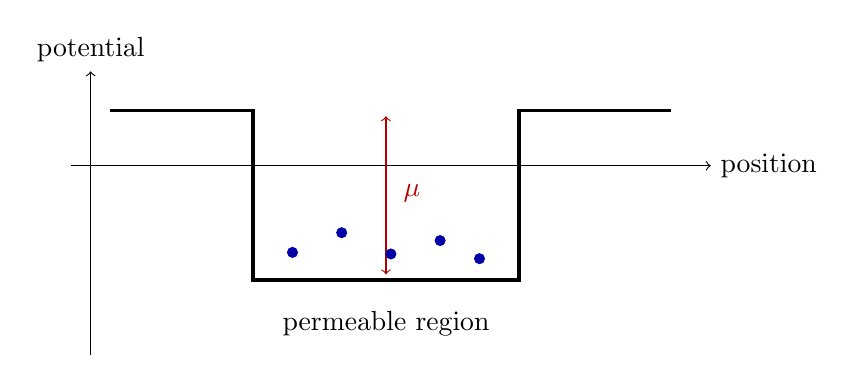
\begin{tikzpicture}[x=1.25cm,y=1.0cm]
\draw[->] (-3.2,0) -- (3.3,0) node[right] {position};
\draw[->] (-3.0,-2.4) -- (-3.0,1.2) node[above] {potential};
\draw[very thick] (-2.8,0.7) -- (-1.35,0.7)
 -- (-1.35,-1.45) -- (1.35,-1.45) -- (1.35,0.7) -- (2.9,0.7);
\draw[<->,red!70!black] (0,0.63) -- (0,-1.38);
\node[right,red!70!black] at (0.08,-0.35) {$\mu$};
\foreach \x/\y in {-0.95/-1.1,-0.45/-0.85,0.05/-1.12,0.55/-0.95,0.95/-1.18}
  \fill[blue!65!black] (\x,\y) circle (2pt);
\node at (0,-2.0) {permeable region};
\end{tikzpicture}
}
\caption{Modifier le décalage du potentiel modifie la préférence pour le nombre de particules. Dans la description grand canonique, ce décalage est représenté par le potentiel chimique.}
\end{figure}

Cette expérience de pensée rend le potentiel chimique concret. C’est l’avantage énergétique associé à l’ajout d’une particule par rapport à un réservoir. Si plusieurs espèces peuvent traverser la paroi, chacune possède son propre potentiel chimique. Une enceinte fermée est différente : dans ce cas, \(N\) est fixé et le potentiel chimique est déduit par voie thermodynamique plutôt qu’imposé par un échange avec un réservoir.

\begin{classroomqa}
\audiencequestion{La profondeur du puits est-elle littéralement le potentiel chimique ?}
\lecturerresponse{Elle constitue une réalisation mécanique directe d’une différence de potentiel chimique. Abaisser de \(\mu\) tous les niveaux à une particule à l’intérieur contribue \(-\mu N\) à l’énergie, et donc \(+\beta\mu N\) à l’exposant de Boltzmann. Seules les différences de potentiel chimique comptent. \lecturetimestamp{00:44:49--00:45:40}}
\end{classroomqa}

Puisque les particules peuvent entrer et sortir, la somme de partition doit inclure tous les nombres de particules :
\begin{equation}
\Xi(T,\mu)
=\sum_{N=0}^{\infty}\;\sum_{\mathcal C_N}
\exp\!\left[-\beta E(\mathcal C_N)+\beta\mu N\right].
\label{eq:grand-partition}
\end{equation}
La somme intérieure porte sur les configurations ayant un nombre fixé \(N\) ; la somme extérieure porte sur \(N\) lui-même. Le poids grand canonique peut aussi s’écrire \(e^{-\beta(E-\mu N)}\).

\begin{figure}[ht]
\centering
\includegraphics[width=0.88\textwidth]{lecture_10_figure_08.png}
\caption{L’enceinte perméable et la somme grand canonique sur le nombre de particules et les configurations.}
\lectureframe{00:47:15}
\end{figure}

\begin{classroomqa}
\audiencequestion{Qu’est-ce qui change lorsque l’enceinte est fermée ?}
\lecturerresponse{Le nombre de particules cesse de fluctuer. On utilise alors la fonction de partition canonique à \(N\) fixé. Dans l’enceinte perméable, \(N\) est une variable thermodynamique dont la valeur moyenne est contrôlée par \(\mu\). \lecturetimestamp{00:45:42--00:47:50}}
\end{classroomqa}

À température fixée, faire varier \(\mu\) modifie ordinairement la densité de façon continue. En dessous d’une température critique, cela peut au contraire provoquer un saut brusque. C’est le phénomène fluide que nous cherchons à décrire. Pour obtenir une description microscopique, les particules doivent avoir deux propriétés : elles ne doivent pas pouvoir occuper le même emplacement et elles doivent s’attirer à courte portée.

\section{Des spins à un gaz sur réseau}

Conservons le réseau, mais réinterprétons ses deux états. Définissons un nombre d’occupation
\begin{equation}
n_i=\frac{1+\sigma_i}{2}
=
\begin{cases}
0,&\sigma_i=-1,\\
1,&\sigma_i=+1.
\end{cases}
\label{eq:occupation-map}
\end{equation}
Un site vide correspond à un spin orienté vers le bas ; un site occupé, à un spin orienté vers le haut. Comme \(n_i\) ne peut valoir que zéro ou un, la double occupation est interdite. Le réseau fournit donc lui-même le cœur dur.

\begin{figure}[ht]
\centering
\includegraphics[width=0.84\textwidth]{lecture_10_figure_04.png}
\caption{L’identification au gaz sur réseau commence par \(\sigma=-1\) comme site vide ; \(\sigma=+1\) correspond alors à un site occupé.}
\lectureframe{00:53:45}
\end{figure}

Partons du réseau vide, où tous les spins valent \(\sigma=-1\). Toutes les liaisons sont alignées et ont une énergie \(-J\). Cette énergie constante du vide peut être soustraite. Plaçons maintenant une particule sur un site en deux dimensions. Le spin correspondant s’inverse et prend la valeur \(+1\), ce qui rompt quatre liaisons. Chaque liaison rompue coûte \(2J\), donc
\begin{equation}
\Delta E_1=4(2J)=8J.
\label{eq:one-particle-cost}
\end{equation}
Deux particules éloignées l’une de l’autre rompent huit liaisons et coûtent \(16J\). Si elles occupent des sites voisins, la liaison qui les relie est de nouveau alignée. Seules six liaisons en bordure sont rompues, et le coût est
\begin{equation}
\Delta E_{2,\rm adjacent}=6(2J)=12J.
\end{equation}
Rapprocher les particules abaisse donc l’énergie de
\begin{equation}
16J-12J=4J.
\label{eq:lattice-attraction}
\end{equation}
Le dénombrement présenté à l’oral a d’abord été décrit comme une économie de \(2J\), puis corrigé : une liaison partagée supprime deux contributions de bord rompues, de sorte que l’attraction vaut \(4J\).

\begin{figure}[ht]
\centering
\includegraphics[width=0.84\textwidth]{lecture_10_figure_05.png}
\caption{Dénombrement des liaisons en deux dimensions : une particule isolée coûte \(8J\), deux particules éloignées coûtent \(16J\) et deux particules adjacentes coûtent \(12J\).}
\lectureframe{01:00:25}
\end{figure}

Le gaz sur réseau possède désormais les deux propriétés moléculaires requises. L’occupation binaire assure l’exclusion de cœur dur, et l’interaction d’échange fournit une attraction entre plus proches voisins d’intensité \(4J\). Le nombre de particules peut fluctuer, car les retournements de spin modifient le nombre de sites occupés.

\subsection{Le dictionnaire algébrique exact}

Le dénombrement des liaisons suffit à saisir la physique, mais le changement exact de variables rend l’équivalence manifeste. Substituons
\begin{equation}
\sigma_i=2n_i-1
\end{equation}
dans l’équation~\eqref{eq:ising-hamiltonian}. Pour une liaison,
\begin{equation}
\sigma_i\sigma_j
=4n_in_j-2n_i-2n_j+1.
\end{equation}
Sur un réseau régulier à \(d\) dimensions,
\begin{equation}
\sum_{\langle ij\rangle}(n_i+n_j)=2d\sum_i n_i.
\end{equation}
On obtient donc
\begin{align}
\mathcal H
&=-4J\sum_{\langle ij\rangle}n_in_j
+(4dJ+2h)\sum_i n_i+\text{constant}.
\label{eq:ising-as-lattice-gas}
\end{align}
Comparons avec l’hamiltonien usuel du gaz sur réseau
\begin{equation}
\mathcal H_{\rm lg}
=-\epsilon\sum_{\langle ij\rangle}n_in_j
-\mu\sum_i n_i+\text{constant}.
\label{eq:lattice-gas-hamiltonian}
\end{equation}
Le dictionnaire est
\begin{equation}
\boxed{\epsilon=4J,\qquad
\mu=-(4dJ+2h).}
\label{eq:chemical-potential-map}
\end{equation}

\begin{figure}[ht]
\centering
\includegraphics[width=0.88\textwidth]{lecture_10_figure_09.png}
\caption{Les termes d’échange et de champ à côté du dénombrement énergétique des particules. Le champ modifie l’énergie d’insertion sans changer l’attraction entre plus proches voisins.}
\lectureframe{01:04:30}
\end{figure}

En deux dimensions, l’insertion d’une particule isolée modifie l’énergie de
\begin{equation}
8J+2h=-\mu.
\end{equation}
Le terme \(8J\) provient des liaisons rompues ; \(2h\) provient du retournement d’un spin, de \(-1\) à \(+1\). Modifier \(h\) revient donc à modifier le potentiel chimique, tandis que l’attraction \(4J\) reste fixe. Le champ n’est pas littéralement égal à \(\mu\), car le niveau de référence d’échange apporte le décalage \(4dJ\).

\begin{classroomqa}
\audiencequestion{Si le champ contrôle le nombre de particules, pourquoi \(h\) n’est-il pas simplement le potentiel chimique ?}
\lecturerresponse{La création d’une particule rompt aussi des liaisons d’échange par rapport à l’état de référence vide. Le coefficient usuel de \(-N\) est donc \(\mu=-(4dJ+2h)\), et non simplement \(-2h\). Le décalage dépend de \(J\) et du nombre de coordination. \lecturetimestamp{01:06:28--01:06:41}}
\end{classroomqa}

La densité est tout aussi simple :
\begin{equation}
\rho=\expect{n_i}
=\frac{1+\expect{\sigma_i}}{2}
=\frac{1+m}{2}.
\label{eq:density-map}
\end{equation}
Ainsi, \(m=-1\) correspond au réseau vide, \(m=+1\) au réseau complètement rempli, et \(m=0\) au demi-remplissage. Le nombre total de particules est \(N_{\rm p}=\sum_i n_i\) ; la densité est \(N_{\rm p}/N\).

\begin{figure}[ht]
\centering
\includegraphics[width=0.90\textwidth]{lecture_10_figure_10.png}
\caption{La relation entre densité \(\rho=(1+m)/2\) et aimantation, à côté de la ligne de coexistence magnétique.}
\lectureframe{01:08:25}
\end{figure}

\begin{classroomqa}
\audiencequestion{\((1+m)/2\) désigne-t-il le nombre de particules ou la densité ?}
\lecturerresponse{C’est l’occupation moyenne par site, donc la densité du réseau, sans dimension. La multiplication par le nombre total de sites donne le nombre moyen de particules. Il est important de distinguer une densité intensive d’un dénombrement extensif. \lecturetimestamp{01:06:43--01:09:31}}
\end{classroomqa}

\section{Le diagramme de phases magnétique devient celui du fluide}

Transposons la figure~\ref{fig:ising-phase-plane} à l’aide des équations~\eqref{eq:chemical-potential-map} et \eqref{eq:density-map}. Au-dessus de \(T_c\), faire varier \(\mu\) modifie la densité de façon continue. En dessous de \(T_c\), le franchissement de la valeur de coexistence
\begin{equation}
\mu_{\rm coex}=-4dJ
\qquad(h=0)
\label{eq:coexistence-mu}
\end{equation}
fait sauter la densité entre un gaz dilué et un liquide dense. À \(T_c\), les deux densités se confondent et la discontinuité disparaît.

\begin{figure}[ht]
\centering
\includegraphics[width=0.92\textwidth]{lecture_10_figure_11.png}
\caption{La ligne de coexistence d’Ising interprétée comme un diagramme de phases liquide--gaz. Le gaz se trouve du côté des faibles densités, le liquide du côté des fortes densités, et l’on peut passer continûment de l’un à l’autre en contournant l’extrémité critique.}
\lectureframe{01:14:30}
\end{figure}

\begin{figure}[ht]
\centering
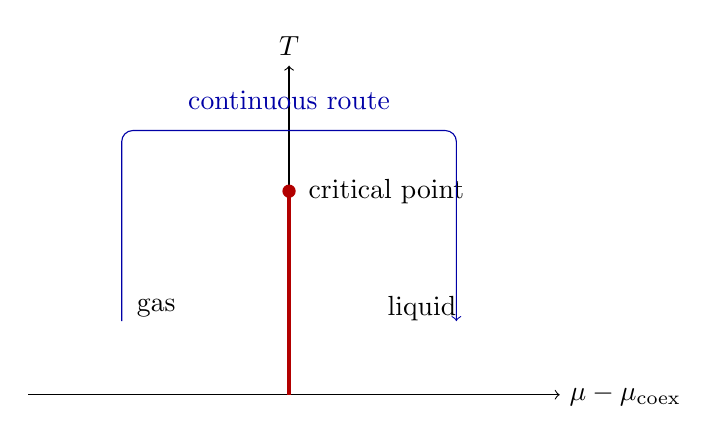
\begin{tikzpicture}[x=1.25cm,y=1.1cm]
\draw[->] (-2.65,0) -- (2.75,0) node[right] {$\mu-\mu_{\rm coex}$};
\draw[->] (0,0) -- (0,3.8) node[above] {$T$};
\draw[very thick,red!70!black] (0,0) -- (0,2.35);
\fill[red!70!black] (0,2.35) circle (2.4pt);
\node[right] at (0.1,2.35) {critical point};
\node at (-1.35,1.0) {gas};
\node at (1.35,1.0) {liquid};
\draw[->,blue!65!black,rounded corners]
 (-1.7,0.85) -- (-1.7,3.05) -- (1.7,3.05) -- (1.7,0.85);
\node[blue!65!black] at (0,3.4) {continuous route};
\end{tikzpicture}
\caption{Le liquide et le gaz sont des phases distinctes en dessous de l’extrémité, mais aucune frontière singulière ne les sépare dans la région supercritique.}
\label{fig:liquid-gas-plane}
\end{figure}

On retrouve ainsi la ligne d’ébullition familière. À pression fixée, chauffer un liquide jusqu’à ce qu’il franchisse la coexistence provoque l’ébullition. À température fixée, faire varier la pression ou le potentiel chimique peut aussi faire franchir la même frontière. Une vapeur surchauffée ou un liquide surfondu constitue le prolongement métastable au-delà de la coexistence à l’équilibre ; la description de sa durée de vie nécessite une dynamique de nucléation, qui dépasse le cadre de cette construction à l’équilibre.

\begin{classroomqa}
\audiencequestion{La vapeur surchauffée est-elle représentée dans ce diagramme de phases ?}
\lecturerresponse{Le diagramme d’équilibre indique la frontière de coexistence. Un état surchauffé ou sursaturé est métastable : il persiste temporairement du mauvais côté parce que la formation d’une gouttelette critique a un coût d’énergie libre interfaciale. Nous ne calculons pas ici ce raffinement cinétique. \lecturetimestamp{01:12:19--01:12:29}}
\end{classroomqa}

\begin{classroomqa}
\audiencequestion{Comment fait-on varier le potentiel chimique dans un fluide ordinaire ?}
\lecturerresponse{L’enceinte avec son puits de potentiel constitue le dispositif de contrôle théorique le plus simple. En laboratoire, on fait plus souvent varier la pression ou le volume, ou bien le contact avec un réservoir ; la thermodynamique traduit alors ces contrôles en une variation du potentiel chimique. \lecturetimestamp{01:12:30--01:13:59}}
\end{classroomqa}

\begin{classroomqa}
\audiencequestion{Lorsque la densité change, modifie-t-on le potentiel moléculaire \(J\) ?}
\lecturerresponse{Non. Pour une substance donnée, \(J\) représente l’attraction à courte portée et reste fixe dans ce modèle. Modifier \(\mu\) change le nombre de sites occupés et donc la distribution des distances intermoléculaires. Modifier \(J\) reviendrait à changer la substance ou l’interaction microscopique. \lecturetimestamp{01:14:50--01:15:41}}
\end{classroomqa}

\begin{classroomqa}
\audiencequestion{La température critique est-elle la même chose que le point d’ébullition ordinaire ?}
\lecturerresponse{Non. Le point d’ébullition est défini à une pression choisie ; il se déplace donc le long de la courbe de coexistence lorsque la pression varie. La température critique est l’unique extrémité au-dessus de laquelle le liquide et le gaz ne sont plus séparés par une frontière de phase. La pression n’a pas été explicitement déduite dans ce traitement du gaz sur réseau. \lecturetimestamp{01:15:42--01:17:02}}
\end{classroomqa}

On peut maintenant énoncer le résultat central. L’aimant d’Ising et le gaz sur réseau ne se contentent pas de présenter des diagrammes semblables. Ils partagent la même fonction de partition après un changement de variables et de paramètres. À chaque propriété thermodynamique singulière de l’un correspond une propriété de l’autre :
\begin{equation}
\begin{array}{c|c}
\text{Ising magnet} & \text{lattice gas}\\ \hline
\sigma_i=\pm1 & n_i=0,1\\
m=\expect{\sigma} & \rho=(1+m)/2\\
h & \mu=-(4dJ+2h)\\
\text{aligned exchange} & \text{nearest-neighbor attraction}\\
h=0,\ T<T_c & \text{liquid--gas coexistence}\\
(T_c,0) & \text{critical endpoint}
\end{array}
\label{eq:ising-fluid-dictionary}
\end{equation}

\section{Exposants critiques et universalité}

Au voisinage d’un point critique, les grandeurs thermodynamiques présentent souvent des singularités en loi de puissance. Avec la température réduite
\begin{equation}
t=\frac{T-T_c}{T_c},
\end{equation}
on écrit schématiquement
\begin{equation}
m\sim(-t)^{\beta_{\rm crit}},
\qquad
\chi\sim |t|^{-\gamma},
\qquad
\xi\sim |t|^{-\nu}.
\label{eq:critical-exponents}
\end{equation}
Ici, \(\beta_{\rm crit}\) est un exposant critique, et non l’inverse de la température. Le champ moyen donne \(\beta_{\rm crit}=1/2\), mais les fluctuations modifient les exposants en dessous de la dimension critique supérieure.

Les exposants ne sont pas nécessairement entiers. Ils ne sont pas non plus tous irrationnels : le modèle d’Ising bidimensionnel possède notamment plusieurs exposants rationnels exacts, tandis que les valeurs du modèle tridimensionnel sont non triviales et déterminées avec grande précision par la théorie et le calcul. La leçon générale est que les exposants ne sont généralement pas fixés par une analyse dimensionnelle élémentaire.

Plus remarquable encore, les détails microscopiques ne les déterminent souvent pas. Des systèmes de même dimension spatiale, présentant la même symétrie du paramètre d’ordre et des interactions suffisamment courtes, peuvent s’écouler vers la même théorie critique à grande distance. Ils appartiennent à une même classe d’\emph{universalité}. Un aimant uniaxial et l’extrémité liquide--gaz ordinaire ont tous deux un paramètre d’ordre scalaire unique et appartiennent à la classe d’universalité d’Ising dans une même dimension.

\begin{classroomqa}
\audiencequestion{Les classes d’universalité forment-elles une liste finie ou discrète ?}
\lecturerresponse{Il existe de nombreuses classes, organisées selon la dimension, les symétries, les lois de conservation, la portée des interactions et d’autres propriétés à grande distance. Dans bien des cas familiers, les points fixes et les ensembles d’exposants sont discrets, mais il existe aussi des systèmes dont les exposants varient de façon continue. Il est prudent de ne pas prétendre que le catalogue est fini ; de nombreux systèmes microscopiquement différents partagent les mêmes propriétés à grande distance. \lecturetimestamp{01:18:50--01:19:38}}
\end{classroomqa}

\begin{classroomqa}
\audiencequestion{Si le liquide et le gaz coexistent, qu’est-ce qui les sépare dans un récipient réel ?}
\lecturerresponse{Une interface les sépare. La tension superficielle pénalise l’aire interfaciale, tandis que la gravité crée un gradient vertical de potentiel chimique et place généralement le liquide, plus dense, sous le gaz. Lorsque la gravité est négligeable, la géométrie est déterminée plus directement par la tension superficielle et les conditions aux limites. \lecturetimestamp{01:19:40--01:21:18}}
\end{classroomqa}

\begin{classroomqa}
\audiencequestion{Où se trouve la chaleur de vaporisation dans cette représentation ?}
\lecturerresponse{En dessous du point critique, le franchissement de la ligne de coexistence du premier ordre s’accompagne généralement d’une chaleur latente. La chaleur de vaporisation tend vers zéro à mesure que l’on approche de l’extrémité critique, car les deux phases y deviennent identiques. Ce cours établit la structure des phases, mais ne calcule pas la chaleur latente. \lecturetimestamp{01:21:19--01:22:18}}
\end{classroomqa}

\begin{classroomqa}
\audiencequestion{Une transition de phase peut-elle servir de détecteur sensible, par exemple dans un dispositif supraconducteur ?}
\lecturerresponse{Oui. Au voisinage d’une transition, une faible perturbation peut produire une réponse importante ou déclencher un changement d’état. Les détecteurs pratiques exploitent cette sensibilité, même si le paramètre d’ordre et la dynamique concernés peuvent différer de ceux de l’exemple d’Ising. \lecturetimestamp{01:22:19--01:24:05}}
\end{classroomqa}

Le cours de mécanique statistique s’achève ici. Nous sommes partis de l’entropie et de l’équilibre, puis avons étudié les fonctions de partition et les gaz, avant de montrer qu’un aimant et un fluide peuvent être deux descriptions d’un même phénomène critique.

\section{Discussion après le cours : ajustement fin et sélection}

Après la fin du cours formel, la conversation s’est poursuivie pendant environ quarante minutes. Elle mérite d’être conservée, mais il ne faut pas la confondre avec la dérivation qui précède. Le sujet n’est plus le gaz sur réseau, mais la logique de l’ajustement fin et l’usage prudent de la sélection anthropique en cosmologie.

\subsection{Les petites valeurs ne sont pas automatiquement le fruit d’un ajustement fin}

Aucune phrase ne permet de trancher tous les usages de l’expression \emph{principe anthropique}. Le point de départ utile est opérationnel : lorsqu’une théorie autorise de nombreux environnements réalisés, les observations sont conditionnées par le fait que des observateurs ne peuvent apparaître que dans certains d’entre eux. Cet énoncé conditionnel peut être rationnel. Il devient vide si on l’invoque sans ensemble, sans condition de sélection ou sans mécanisme qui donne un sens physique aux différentes possibilités.

Avant d’introduire la sélection, il faut distinguer un petit paramètre d’un paramètre ajusté avec précision. Une valeur peut être petite parce qu’un mécanisme dynamique stable l’entraîne vers une valeur particulière. Il y a ajustement fin lorsque la valeur observée semble exiger un équilibre d’une précision extraordinaire entre des contributions autrement indépendantes, sans mécanisme de rappel connu ni symétrie qui protège cet équilibre.

\begin{classroomqa}
\audiencequestion{Le principe anthropique peut-il être formulé précisément ?}
\lecturerresponse{Son usage défendable est conditionnel, et non mystique : si de nombreux environnements physiquement réalisés ont des paramètres différents, alors les environnements observés par des êtres comme nous sont tirés du sous-ensemble compatible avec la présence d’observateurs. Cela ne crée pas en soi ces environnements et ne leur attribue pas de probabilités ; ces tâches relèvent de la physique sous-jacente. \lecturetimestamp{01:25:45--01:26:13}}
\end{classroomqa}

La constante cosmologique en est l’exemple motivant. Sa valeur observée est extraordinairement faible par rapport aux contributions naïves à l’énergie du vide issues de la théorie quantique des champs. La difficulté ne tient pas seulement à la petitesse de la valeur finale. De nombreux termes importants semblent devoir se compenser avec une précision immense, alors qu’aucun mécanisme de rétroaction accepté à basse énergie ne ramène le résultat vers la valeur observée.

\subsection{Le dirigeable et le sous-marin}

Deux exemples de poussée d’Archimède permettent d’isoler la distinction. Un dirigeable flotte à une altitude où sa masse volumique moyenne égale celle de l’air ambiant. La masse volumique de l’air diminue avec l’altitude. Si le dirigeable s’élève, l’air extérieur devient moins dense et le dirigeable tend à redescendre ; s’il descend, l’air extérieur devient plus dense et le dirigeable tend à remonter. L’égalité des masses volumiques peut être numériquement délicate, mais le gradient atmosphérique fournit une rétroaction de rappel. L’équilibre s’explique par la dynamique.

Un sous-marin en flottabilité neutre dans une eau presque incompressible présente un cas différent. La masse volumique de l’eau varie peu avec la profondeur. Si la masse volumique moyenne du sous-marin se trouve égale à celle de l’eau environnante, aucun mécanisme de rappel comparable, dépendant de la profondeur, n’explique cette égalité. Un écart infime le fait monter ou couler. Obtenir une flottabilité neutre exige de régler avec précision le ballast et le contenu du sous-marin. Le faible écart résiduel relève alors d’un ajustement fin, à moins qu’un système de contrôle ou un mécanisme de conception ne l’explique.

\begin{figure}[ht]
\centering
\resizebox{\linewidth}{!}{%
\begin{tikzpicture}[>=Latex]
\begin{scope}[xshift=-3.8cm]
\shade[top color=blue!5,bottom color=blue!28] (-2.5,-2.2) rectangle (2.5,2.2);
\draw[very thick,rounded corners=18pt,fill=yellow!35]
  (-1.15,0) ellipse (1.15 and 0.55);
\draw[thick] (0,-0.55) -- (0,-1.05);
\draw[thick,fill=gray!20] (-0.45,-1.05) rectangle (0.45,-1.38);
\draw[->,red!70!black,thick] (1.65,1.45) -- (1.65,0.55)
 node[midway,right] {restoring};
\draw[->,red!70!black,thick] (-1.65,-1.45) -- (-1.65,-0.55)
 node[midway,left] {restoring};
\node at (0,2.55) {\textbf{Blimp: density gradient}};
\node[align=center] at (0,-2.75) {displacement changes\\the buoyant imbalance};
\end{scope}
\begin{scope}[xshift=3.8cm]
\shade[top color=cyan!10,bottom color=blue!45] (-2.5,-2.2) rectangle (2.5,2.2);
\draw[very thick,fill=gray!35,rounded corners=12pt]
  (-1.45,-0.25) -- (1.1,-0.25) arc (-90:90:0.38)
  -- (-1.45,0.51) -- cycle;
\draw[thick] (-0.25,0.51) -- (-0.25,0.85) -- (0.35,0.85) -- (0.35,0.51);
\draw[->,red!70!black,thick] (1.65,0.15) -- (1.65,1.35)
 node[midway,right] {rise};
\draw[->,red!70!black,thick] (-1.65,0.15) -- (-1.65,-1.35)
 node[midway,left] {sink};
\node at (0,2.55) {\textbf{Submarine: nearly uniform density}};
\node[align=center] at (0,-2.75) {no depth-dependent feedback\\protects neutral buoyancy};
\end{scope}
\end{tikzpicture}
}
\caption{Un faible écart résiduel peut être stable grâce à la dynamique ou véritablement ajusté. Le dirigeable bénéficie d’une rétroaction de rappel ; dans le modèle idéalisé du sous-marin, il faut ajuster sa masse volumique moyenne à celle de l’eau.}
\label{fig:blimp-submarine}
\end{figure}

\begin{classroomqa}
\audiencequestion{Pourquoi l’équipage du sous-marin devrait-il demander une explication si l’on observe une flottabilité neutre ?}
\lecturerresponse{Parce qu’en l’absence d’un mécanisme de contrôle du ballast, ni une symétrie ni une rétroaction de l’environnement ne protège l’égalité de deux masses volumiques indépendantes. La question n’est pas de savoir si cette égalité est logiquement possible, mais pourquoi le système se trouve dans une région aussi étroite de son espace des paramètres. \lecturetimestamp{01:35:05--01:36:25}}
\end{classroomqa}

\subsection{Domaines multiples et observation conditionnelle}

Imaginons maintenant un processus qui produit un très grand nombre de sous-marins aux masses volumiques moyennes diverses. La plupart coulent ou remontent ; seule une infime fraction subsiste longtemps dans la zone habitable entre la surface et le fond. Un observateur qui vit nécessairement dans l’un des sous-marins survivants ne devrait pas s’étonner de mesurer une flottabilité presque neutre. L’observation est sélectionnée par la condition nécessaire à la présence de l’observateur.

Ce raisonnement requiert deux éléments :
\begin{enumerate}
\item un processus physique qui réalise effectivement de nombreuses possibilités, et non des possibilités qui n’existent que dans l’imagination ;
\item une condition de sélection expliquant pourquoi les observations ne sont faites que dans un sous-ensemble restreint.
\end{enumerate}
La sélection ne remplace pas le mécanisme de production. Une fois l’ensemble constitué, elle modifie la probabilité conditionnelle de ce qu’un observateur mesure.

\begin{classroomqa}
\audiencequestion{L’argument consiste-t-il simplement à dire que, dans un échantillon suffisamment grand, des événements improbables se produisent quelque part ?}
\lecturerresponse{Ce n’est que la première moitié du raisonnement. La seconde est le conditionnement observationnel : les observateurs ne sont pas tirés uniformément parmi tous les domaines, mais uniquement parmi ceux où leur existence est possible. Une proposition complète doit encore fournir une mesure sur les domaines et une explication physique de leur production. \lecturetimestamp{01:39:19--01:40:36}}
\end{classroomqa}

Appliquée à l’énergie du vide, une constante cosmologique fortement négative peut entraîner un effondrement trop rapide de l’Univers, tandis qu’une valeur positive suffisamment grande peut empêcher la matière de se condenser en galaxies. La valeur observée se situe dans la plage étroite compatible avec des structures de longue durée de vie. Cela fournit une condition de sélection possible, et non une dérivation de la distribution des constantes cosmologiques.

La théorie quantique des champs ajoute le problème de l’ajustement fin : les contributions au vide provenant de différents champs et de différentes échelles sont chacune bien supérieures au résidu observé. Si ces termes se compensent presque exactement, le résultat ressemble au sous-marin soigneusement équilibré plutôt qu’au dirigeable autorégulé. L’analogie vise à mettre en évidence le problème logique, pas à le résoudre.

\begin{classroomqa}
\audiencequestion{Des variations d’un paramètre peuvent-elles être compensées par des variations de plusieurs autres ?}
\lecturerresponse{Oui. L’ensemble viable ne forme pas nécessairement un intervalle étroit sur un seul axe ; il peut constituer une surface mince dans un espace des paramètres multidimensionnel. Des variations corrélées peuvent préserver les structures, mais il faut alors se demander pourquoi les paramètres réalisés se trouvent au voisinage de cette surface et quelle mesure la théorie sous-jacente lui attribue. \lecturetimestamp{01:45:10--01:46:19}}
\end{classroomqa}

\begin{figure}[ht]
\centering
\begin{tikzpicture}[x=1.3cm,y=1.05cm,>=Latex]
\draw[->] (-3.2,0) -- (3.4,0) node[right] {$\lambda_1$};
\draw[->] (0,-2.5) -- (0,2.65) node[above] {$\lambda_2$};
\fill[gray!12] (-3,-2.25) rectangle (3.1,2.3);
\draw[very thick,blue!65!black]
 (-2.8,-1.55) .. controls (-1.3,-0.75) and (0.15,0.05) .. (2.85,1.55);
\draw[very thick,blue!25]
 (-2.8,-1.25) .. controls (-1.3,-0.45) and (0.15,0.35) .. (2.85,1.85);
\fill[blue!15,opacity=.65]
 (-2.8,-1.55) .. controls (-1.3,-0.75) and (0.15,0.05) .. (2.85,1.55)
 -- (2.85,1.85) .. controls (0.15,0.35) and (-1.3,-0.45) .. (-2.8,-1.25) -- cycle;
\node[blue!65!black,rotate=28] at (1.3,0.95) {viable band};
\foreach \x/\y in {-2.4/1.45,-1.7/-1.8,-0.9/1.8,0.3/-1.45,1.2/1.85,2.4/-0.8}
  \fill[red!65!black] (\x,\y) circle (2pt);
\fill[green!45!black] (0.55,0.58) circle (2.8pt);
\node[green!35!black,right] at (0.65,0.55) {observed domain};
\end{tikzpicture}
\caption{Avec plusieurs paramètres, l’habitabilité ou la viabilité des structures peut occuper une bande étroite où les paramètres sont corrélés, plutôt qu’un intervalle étroit pour un seul paramètre. La sélection restreint les observations à cette bande, mais ne produit pas la distribution des paramètres.}
\label{fig:viable-parameter-band}
\end{figure}

\subsection{Propositions de paysage et incertitudes associées}

Une théorie comportant de nombreux vides métastables, éventuellement peuplés dans différents domaines cosmologiques, pourrait fournir ces possibilités. Les idées de paysage en théorie des cordes et les scénarios d’inflation éternelle en sont des exemples, mais leur réalisation détaillée et la mesure de probabilité associée restent incertaines. Le cours présente cette piste comme une possibilité, pas comme un fait établi.

Une symétrie fournirait une explication plus conventionnelle si elle imposait l’annulation exacte de la constante cosmologique. La difficulté est que l’expansion accélérée observée correspond à une valeur petite, mais non nulle. Un mécanisme qui donne naturellement une valeur exactement nulle n’explique pas automatiquement un faible résidu ; la brisure de symétrie peut simplement réintroduire l’ajustement fin. L’image du sous-marin revient ici : une corde pourrait le maintenir à la profondeur voulue, mais il faudrait alors identifier le mécanisme que constitue cette corde, et non le supposer.

\begin{classroomqa}
\audiencequestion{Mesurer un paramètre avec une très grande précision viole-t-il le principe d’incertitude ?}
\lecturerresponse{Non. Une relation d’incertitude porte sur des paires données d’observables qui ne commutent pas. Une constante de couplage ou un paramètre du vide peut avoir une valeur bien définie sans être la variable conjuguée canonique d’une observable non contrôlée. À elle seule, la précision ne crée aucun paradoxe lié au principe d’incertitude. \lecturetimestamp{01:49:21--01:49:36}}
\end{classroomqa}

\begin{classroomqa}
\audiencequestion{Le raisonnement anthropique explique-t-il la valeur, ou se contente-t-il de répéter qu’elle est nécessaire aux observateurs ?}
\lecturerresponse{La sélection à elle seule n’est pas une explication dynamique. Son rôle légitime est de modifier les probabilités conditionnelles dans un ensemble réalisé physiquement. Employée sans ensemble, sans mesure ni conséquences vérifiables, elle risque de devenir une étiquette plutôt qu’une explication. \lecturetimestamp{01:49:37--01:50:21}}
\end{classroomqa}

\subsection{Coïncidences modérées en physique des particules}

Tous les paramètres importants pour la vie ne sont pas ajustés avec la même précision extraordinaire. La matière ordinaire dépend des photons, des électrons, des quarks légers et de l’interaction forte ; les neutrinos influent sur la cosmologie, mais ne sont pas les agents directs de la liaison des atomes. La différence de masse entre le proton--neutron est particulièrement déterminante. Le neutron étant légèrement plus lourd que le proton, les neutrons isolés peuvent se désintégrer et l’hydrogène ordinaire est stable. Inverser suffisamment cet ordre modifierait profondément la chimie nucléaire.

La masse de l’électron et la constante de structure fine déterminent elles aussi les dimensions des atomes et leurs énergies de liaison. Les modifier substantiellement changerait la chimie. Ces énoncés de sensibilité sont pertinents, mais il ne faut pas les exagérer au point d’affirmer que toute faible variation interdit toute forme imaginable de complexité. Comparées au problème de la constante cosmologique, nombre de ces coïncidences sont modérées et corrélées à d’autres paramètres.

La hiérarchie associée à l’échelle électrofaible constitue un autre problème majeur de naturalité : les contributions radiatives tendent à rendre la masse d’un scalaire fondamental sensible aux hautes échelles, à moins qu’une structure supplémentaire ne la protège. Son statut et son interprétation diffèrent de ceux du problème de l’énergie du vide ; aucun des deux ne doit être réduit à un slogan.

\begin{classroomqa}
\audiencequestion{La différence de masse entre le proton--neutron compte-t-elle vraiment pour la matière ordinaire ?}
\lecturerresponse{Oui. L’ordre observé permet à l’hydrogène d’être stable et détermine la stabilité bêta des noyaux. Des variations modestes peuvent réorganiser les abondances nucléaires et la combustion stellaire. Une analyse rigoureuse doit faire varier les paramètres couplés de manière cohérente, au lieu de modifier une valeur en maintenant toutes les autres fixes. \lecturetimestamp{01:51:47--01:53:08}}
\end{classroomqa}

\begin{classroomqa}
\audiencequestion{Quel rôle jouent la masse de l’électron et la constante de structure fine ?}
\lecturerresponse{Elles déterminent les échelles caractéristiques d’énergie et de longueur atomiques, schématiquement \(E_{\rm atom}\sim \alpha^2m_e\) et \(a_0\sim(\alpha m_e)^{-1}\) dans les unités \(\hbar=c=1\). Des variations importantes remanieraient la chimie, même si la région exacte des valeurs viables relève d’un problème multidimensionnel. \lecturetimestamp{01:53:09--01:54:12}}
\end{classroomqa}

\subsection{Désaccords, dépendance temporelle et tests}

La discussion aborde brièvement les critiques de l’inflation et l’interprétation des données cosmologiques de précision. Ce désaccord historique doit être présenté comme tel, sans prétendre le trancher par la rhétorique. L’inflation possède des prédictions phénoménologiques qui ont été confirmées et de nombreuses variantes de modèles ; les questions relatives aux conditions initiales, aux mesures et à la testabilité restent ouvertes. Les données contraignent les modèles, mais une simple référence à une expérience dans une conversation ne permet pas de trancher l’ensemble du cadre théorique.

\begin{classroomqa}
\audiencequestion{La constante cosmologique pourrait-elle varier lentement avec le temps au lieu d’être constante ?}
\lecturerresponse{Un champ dynamique d’énergie noire peut produire une accélération qui dépend du temps. Il introduit un potentiel et des conditions initiales qu’il faut eux-mêmes expliquer, et les observations contraignent l’équation d’état à rester proche de celle d’une constante cosmologique. Dans la discussion à l’époque du cours, aucun élément n’exigeait une variation temporelle appréciable. \lecturetimestamp{01:57:17--01:59:19}}
\end{classroomqa}

\begin{classroomqa}
\audiencequestion{La sélection anthropique fait-elle apparaître par nucléation différents univers ou domaines ?}
\lecturerresponse{Non. La sélection indique quels domaines réalisés peuvent contenir des observateurs ; elle ne crée pas ces domaines. Il faudrait qu’un mécanisme cosmologique distinct les produise, par exemple des transitions entre vides au cours d’une histoire inflationnaire. \lecturetimestamp{01:59:20--01:59:42}}
\end{classroomqa}

L’ordre causal doit rester clair :
\begin{equation}
\begin{gathered}
\text{laws and initial conditions}\\[-0.15em]
\downarrow\\[-0.15em]
\text{physical environments}\\[-0.15em]
\downarrow\\[-0.15em]
\text{observers and observations}
\end{gathered}
\end{equation}
Les observateurs ne remontent pas le temps pour dicter les lois. Le conditionnement intervient lorsque nous demandons ce qu’un observateur tiré parmi les environnements réalisés est susceptible de mesurer.

La question scientifique n’est donc pas de savoir si le discours paraît philosophique, politique ou religieux. Elle est de déterminer si la proposition définit un ensemble physique, une mesure calculable ou du moins contrainte, et des conséquences susceptibles de la distinguer des autres possibilités. Parmi les signatures possibles évoquées pour la cosmologie à multivide figurent des traces de collisions entre domaines-bulles. Ces signaux sont difficiles à prédire de manière robuste et, au moment de la discussion à l’époque du cours, aucun n’avait été établi dans le fond diffus cosmologique. L’absence d’un test facile constitue une limite sérieuse ; elle ne permet ni de déclarer l’idée vraie ni d’écarter le problème d’ajustement fin sous-jacent.

\begin{classroomqa}
\audiencequestion{Qu’est-ce qui ferait de cet argument de sélection une théorie scientifique ?}
\lecturerresponse{La proposition doit comporter un mécanisme qui produit les différentes possibilités, une mesure de probabilité ou un substitut contrôlé, ainsi que des conséquences observables. Les signatures de collisions entre bulles constituent une piste possible, mais leur absence ou leur ambiguïté montre à quel point le problème de la testabilité est exigeant. \lecturetimestamp{02:02:31--02:04:12}}
\end{classroomqa}

L’échange après le cours s’achève sur cette remarque mesurée. L’ajustement fin indique qu’une explication peut manquer. La symétrie, l’ajustement dynamique et la sélection environnementale sont des explications possibles, mais logiquement distinctes. La sélection peut être rationnelle, mais seulement comme élément d’une explication physique dont les hypothèses et les limites sont énoncées ouvertement.
